\chapter{Реализация параллельной генерации состояний}
\label{cha:parmpi}

\section{Выбор средств распараллеливания}
\label{sec:paral-selection}

\section{Взаимодействие узлов}
\label{sec:mpi-interaction}

\subsection{Сравнение примитивов обмена сообщениями в MPI}
\label{sec:mpi-primitives}

\subsection{Схема асинхронного обмена сообщениями}
\label{sec:async-mpi-queue}

\begin{figure}[ht]
  \centering
  \includegraphics[width=1.0\textwidth]{../../graphics/mpi-async-seq}  
  \caption{Асинхронное взаимодействие узлов (MPI)}
  \label{fig:mpi-async-seq}
\end{figure}

\section{Распределенное завершение}
\label{sec:distributed-termination}

\subsection{Алгоритм Дейкстры}
\label{sec:distr-term-dijkstra}

\begin{figure}[ht]
  \centering
  \includegraphics[width=1\textwidth]{../../graphics/distr-termination}  
  \caption{Распределенное завершение}
\label{fig:dist-term}
\end{figure}

\chapter{Хранение состояний в памяти}
\label{cha:state-store}

\section{Полное хэширование}
\label{sec:fullstate}

\begin{figure}[ht]
  \centering
  \includegraphics[width=1\textwidth]{../../graphics/fullstate}
  
  \caption{Полное хэширование}
  \label{fig:fullstate}
\end{figure}

\section{Битовое хэширование}
\label{sec:buthash}

\begin{figure}[ht]
  \centering
  \includegraphics[width=0.7\textwidth]{../../graphics/bitstate}  
  \caption{Битовое хэширование}
  \label{fig:bitstate}
\end{figure}

\section{Локальная и сетевая очереди состояний}
\label{sec:local-network-queue}


\section{Представление состояния}
\label{sec:state-represent}

\begin{figure}[ht]
  \centering
  \includegraphics[width=0.3\textwidth]{../../graphics/state-representation}  
  \caption{Представление состояний}
  \label{fig:state-repr}
\end{figure}

\chapter{Генерация кода из описания модели}
\label{cha:code-gen}

\section{Выбор используемой нотации}
\label{sec:notation-choice}

\section{Схема процесса верификации}
\label{sec:idef0-codegen}

\begin{figure}[ht]
  \centering
  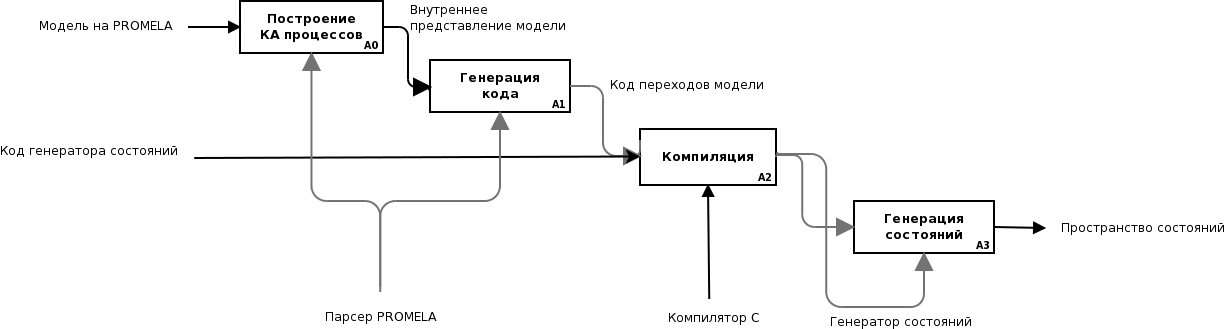
\includegraphics[width=1\textwidth]{../../graphics/idef0-codegen}  
  \caption{Схема процесса верификации}
\label{fig:idef0-codegen}
\end{figure}

%%% Local Variables: 
%%% mode: latex
%%% TeX-master: "main"
%%% End: 
